\documentclass{article}
\usepackage{graphicx}
\usepackage[utf8]{inputenc}
\usepackage[T1]{fontenc}
\usepackage[francais]{babel}
\usepackage{layout}
\usepackage{caption}
\usepackage{subcaption}

\begin{document}
\begin{titlepage}
\begin{center}
\Huge Rapport TPA phase 2

\normalsize
\vspace{0.5cm}
\Large {\underline{ Groupe 3 Bleu : Sokoban} }

\vspace{1cm}

\normalsize
Goron Nathan, De La Rosa Louis-David, Basset Emilien, Demé Quentin

\vspace{1cm}
\begin{center}
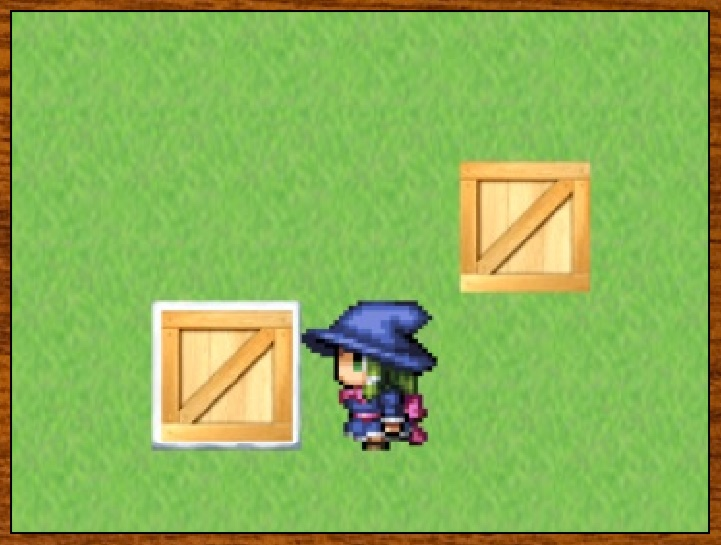
\includegraphics[scale=0.7]{img/main.jpg}
\end{center}
\vspace{3.5cm}
L2 informatique 2016-2017 Université de Caen Basse-Normandie
\end{center}
\end{titlepage}

\newpage
\tableofcontents

\newpage
\begin{center}
	\section{Introduction}
\end{center}

\newpage
\begin{center}
	\section{Cahier des Charges}
	
		\subsection{Résumé des objectifs:}
		\subsection{Librairies utilisées:}
		\subsection{Pré-requis d'utilisation}version logiciel , sys d'exploitation et materiel (souris clavier toussa)
		\subsection{Dates fixées}
		\subsection{Recensement des fonctionnalités}
			\subsubsection{Fonctionnalités obligatoires}
			\subsubsection{Fonctionnalités additionnelles}
		\subsection{Priorités , importance relative des fonctionnalités}
\end{center}

\newpage
\begin{center}
	\section{Explication du programme , détails de conception}
		\subsection{Moteur de jeu}
		\subsection{Algorithme de résolution A* et heuristique}
		\subsection{Interface graphique}
\end{center}

\newpage
\begin{center}
	\section{Schéma UML : diagramme de classe}
\end{center}

\newpage
\begin{center}
	\section{Tests}
		\subsection{Tests de fonctionnement du programme}
		\subsection{Tests de perfrmance de la resolution automatique}
\end{center}

\newpage
\begin{center}
	\section{Conclusion , difficultés rencontrées}
\end{center}

\newpage
\begin{center}
	\section{Bibliographies , sources}
\end{center}







\end{document}